\subsection{Slope Compensation} \label{sec:solution_subsec:slopecompensation}
The extra negative slope is equivalently an extra positive slope on the current ramp. It improves SNR of the sensed inductor current by enhancing the signal as shown in Fig. \ref{sc1}. Hence the stability of the inner-current loop.

\begin{figure}
\begin{minipage}{0.32\textwidth}
    \centering
    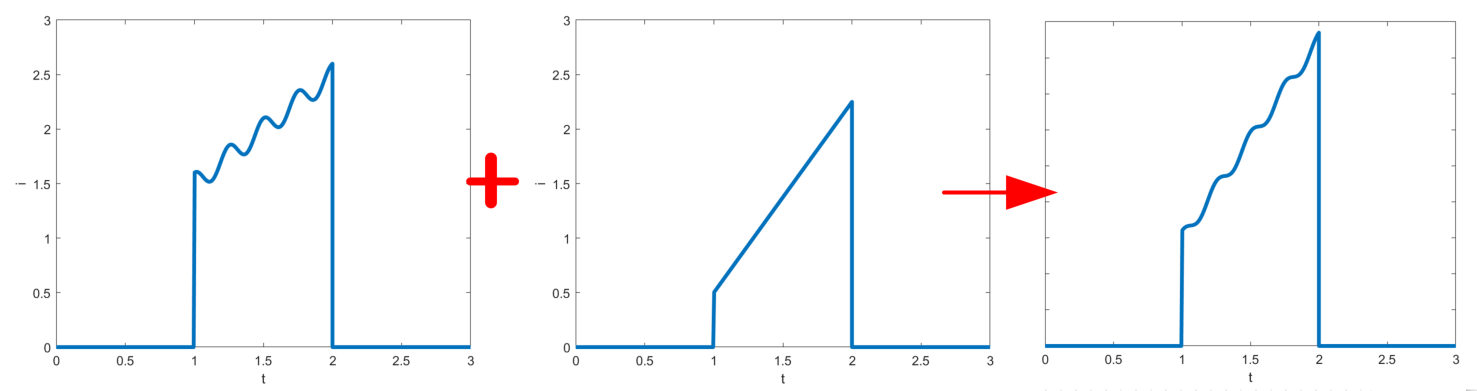
\includegraphics[width=\textwidth]{Figure/section3/slopecompensation/slopecomp.png}
    \caption{ \label{fig:sc1} Mechanism of slope compensation.}
\end{minipage}
~
\begin{minipage}{0.32\textwidth}
    \centering
    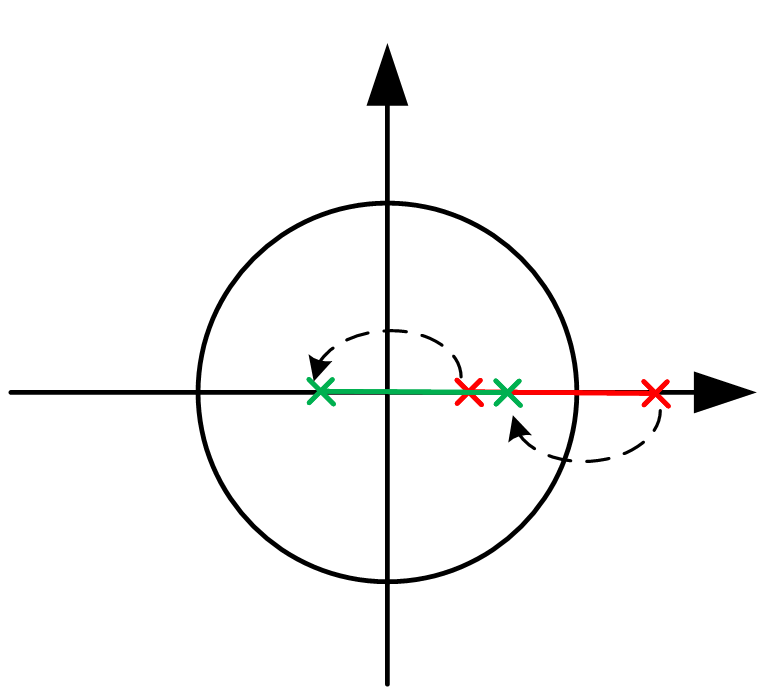
\includegraphics[width=\textwidth]{Figure/section3/slopecompensation/slopecomppole.PNG}
  \caption{  \label{fig:sc2} Pole locations under slope compensation.}
\end{minipage}
% ~
% \begin{minipage}{0.32\textwidth}
%     \centering
%     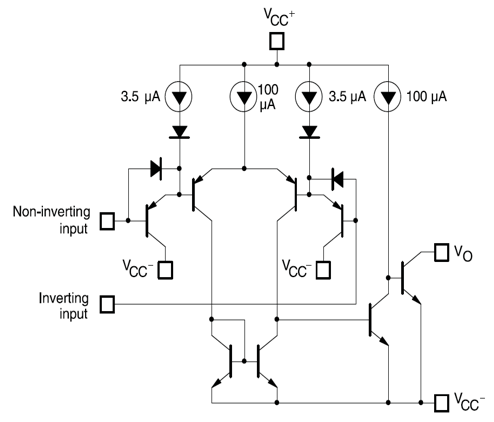
\includegraphics[width=\textwidth]{Figure/section3/copd/physicalmodelcomp.PNG}
%     \caption{\label{fig:physicalmodel} Simplified physical model of a comparator.}
% \end{minipage}
\end{figure}

By the theorem 1, we give the equilibrium existence condition 
\begin{corollary}
$\mathcal{T}$ is an onto-function if and only if the measured inductor current waveform $m_1t+f(t)$ is a strictly monotonic.
\end{corollary}
By the theorem 2, we give the globally asymptotically stability condition 
\begin{corollary}
The $2 \pi f_a f_n > -(m_1/2) t$ if and only if the current command block is globally asymptotically stable.
\end{corollary} 
Performance analysis, by doing linearization and Z-transform
In this method, instead of using constant $i_c[n]$ in every switching cycle, we use $i_c[n] - m_s t$ where $m_s>0$. The inner loop dynamics can be expressed as:
\begin{align}
i_p[n] &= i_p[n-1] - m_2t_{\text{off}} +m_1t_{\text{on}}[n], \\
i_c [n]  &= i_p[n] +f(t_{\text{on}}[n]) + m_s (t_{\text{on}}[n]).
\end{align}
The small-signal model is:
\begin{align}
\tilde i_p[n] &= \tilde i_p[n-1] +  m_1 \tilde t_{\text{on}}[n], \\
\tilde i_c [n] - m_s \tilde t_{\text{on}} [n] & = \tilde i_p[n] + f(t_{\text{on}}[n]) - f(T_{\text{on}}).
\end{align}
Then the new nonlinear static function is $\psi(y) = m_1 \phi ^{-1}(y-f(T_{\text{on}}))$, where $\phi(x) = m_s x + f(x)$. If (\ref{sc1}) holds, we can confidently say the oscillation cannot sustain in the inner loop. 
\begin{align} \label{sc1}
m_s + (f')_{\text{min}} > -m_1/2
\end{align}


To study the influence of $m_s$ the to the transient response of the dual loop, we linearize the $\psi(y)$,
\begin{align} 
\tilde i_p[n] &= \tilde i_p[n-1] +  m_1 \tilde t_{\text{on}}[n], \\
\tilde i_c [n]  & = \tilde i_p[n-1] + (f^{'}(T_{\text{on}}) +m_s+m_1)\tilde t_{\text{on}} [n].
\end{align}
Define an equivalent local slope $s = f^{'}(T_{\text{on}}) +m_s+m_1$, slope ratio $\beta = m_1/s$, and pole of inner current loop $a = 1-\beta$.
\begin{align}
\tilde i_p[n] &=  \beta \tilde i_c [n] + a \tilde i_p[n-1].
\end{align}
We simply the inner current loop as 
\begin{align} \label{iltf1}
C_2(z) = \frac{\beta }{1-a z^{-1}}
\end{align}
From (\ref{iltf1}), ideally, $\beta = 1$, $a = 0$ and the pole of $C_2(z)$ locates at 0, meaning $C_2(z)$ is deadbeat. 
The larger the $|a^{i}_1|$ is, the longer transient under reference step the inner loop will have.

While the operating points is moving, $a^{i}_1$ is within the range
 $ [1 - m_1/(m_1 + m_s + f^{'}_{\text{min}}), 1-m_1/(m_1 + m_s + f^{'}_{\text{max}})]$. 
\begin{align}
a^i_{1_l} &= 1 - \frac{m_1}{(m_1 + m_s + f^{'}_{\text{min}})} \le a^i_1 \nonumber \\
&\le   a^i_{1_u} = 1 - \frac{m_1}{(m_1 + m_s + f^{'}_{\text{max}})}
\end{align}

Both $a^i_{1_l}$ and $a^i_{1_u}$ are increasing with $m_s$. So the optimal $m_s$ should make $a^i_{1_l} = -a^i_{1_u}$.\\
Define the variation bound of a functional $f$ as $BV(f^{'}) \triangleq f^{'}_{\text{max}}-f^{'}_{\text{min}}$, then the optimal worst-case pole can be expressed as
\begin{align}
a^i_{1_{\text{min}}} &= 1 - \frac{2}{1 + \sqrt{1+\left(\frac{BV(f^{'})}{m_1}\right)^2} + \frac{BV(f^{'})}{m_1}} \le a^i_1 \nonumber \\
&\le a^i_{1_{\text{max}}} = 1 - \frac{2}{1 + \sqrt{1+\left(\frac{BV(f^{'})}{m_1}\right)^2} -\frac{BV(f^{'})}{m_1}}
\end{align}
Here the optimal value of $m_s$ when the interference function $f$ is known is 
\begin{align}
    m_s = -\frac{m_1}{2} - (f^{'}_{\text{max}}+f^{'}_{\text{min}}) + \frac{\sqrt{m_1^2+BV^2(f^{'})}}{2}
\end{align}
In the case when the interference function $f$ is not known but the amplitude is limited by $A$ and bandwidth is limited by $\omega$, 
\begin{align}
    m_s = \sqrt{\left(\frac{m_1}{2}\right)^2+A^2\omega^2} -\frac{m_1}{2} 
\end{align}
Then the optimal worst-case pole can be simplified as
\begin{align}
a^i_{1_{\text{min}}} &= 1 - \frac{2}{1 + \sqrt{1+\left(\frac{2A\omega}{m_1}\right)^2} + \frac{2A\omega}{m_1}} \le a^i_1 \nonumber \\
&\le a^i_{1_{\text{max}}} = 1 - \frac{2}{1 + \sqrt{1+\left(\frac{2A\omega}{m_1}\right)^2} -\frac{2A\omega}{m_1}}
\end{align}
So the settling time is
So we conclude that slope compensation is a good method for the interference function whose derivative's variation bound is small.
% The effect of poles by the ramp compensation

% Formulate an optimization